\chapter{Working with outranking digraphs}
\label{sec:3}

\abstract*{To be written.}

\abstract{To be written.}

\section{Outranking digraph model}
\label{sec:3.1}

In the {\tt outrankingDigraphs} module, the {\tt BipolarOutrankingDigraph} class provides our standard {\bf outranking digraph} constructor. Such an instance represents a {\bf hybrid} object of both, the {\tt PerformanceTableau} type and the {\tt OutrankingDigraph} type. A given object contains hence the following attributes:
\begin{enumerate}
\item A ordered dictionary of decision {\bf actions} describing the potential decision actions or alternatives with {\tt name} and {\tt comment} attributes,
\item A possibly empty ordered dictionary of decision {\bf objectives} with {\tt name} and {\tt comment} attributes, describing the multiple preference dimensions involved in the decision problem, 
\item An ordered dictionary of performance {\bf criteria}, i.e. {\em preferentially independent\/} and {\em non-redundant\/} decimal-valued functions used for measuring the performance of each potential decision action with respect to a decision objective,
\item A double dictionary called {\bf evaluation} gathering performance grades for each decision action or alternative on each criterion function. 
\item The digraph {\bf valuationdomain}, a dictionary with three entries: the {\em minimum\/} ($-1.0$, certainly outranked), the {\em median\/} ($0.0$, indeterminate) and the {\em maximum\/} characteristic value ($+1.0$, certainly outranking),
\item The outranking {\bf relation} : a double dictionary defined on the Cartesian product of the set of decision alternatives capturing the credibility of the pairwise {\em outranking situation\/} computed on the basis of the performance differences observed between couples of decision alternatives on the given family of criteria functions.   
\end{enumerate}

Let us construct, for instance, a random bipolar-valued outranking digraph with seven decision actions denotes $a1$, $a2$, ..., $a7$. We need therefore to first generate a corresponding random performance tableaux (see Listing \ref{list:3.1} below).

\begin{lstlisting}[caption={Generating a random performance tableau},label=list:3.1]
>>> from outrankingDigraphs import *
>>> pt = RandomPerformanceTableau(numberOfActions=7,\
...                               seed=100)   
>>> pt
   *------- PerformanceTableau instance description ------*
    Instance class     : RandomPerformanceTableau
    Seed               : 100
    Instance name      : randomperftab
    Actions            : 7
    Criteria           : 7
    NaN proportion (%) : 6.1
>>> pt.showActions()
  *----- show digraphs actions --------------*
   key:  a1
    name:       action #1
    comment:    RandomPerformanceTableau() generated.
   key:  a2
    name:       action #2
    comment:    RandomPerformanceTableau() generated.
     ...
     ...
   key:  a7
    name:       action #7
    comment:    RandomPerformanceTableau() generated.
\end{lstlisting}

In this example we consider furthermore a family of seven {\bf equisignificant cardinal criteria functions} $g1$, $g2$, ..., $g7$, measuring the performance of each alternative on a rational scale from $0.0$ (worst) to $100.00$ (best). In order to capture the grading procedure's potential uncertainty and imprecision, each criterion function $g1$ to $g7$ admits three performance {\bf discrimination thresholds} of $2.5$, $5.0$ and $80.0$ pts for warranting respectively any indifference, preference or considerable performance difference situation.

\begin{lstlisting}[caption={Inspecting the performance criteria},label=list:3.2]
>>> pt.showCriteria()
  *----  criteria -----*
   g1 'RandomPerformanceTableau() instance'
     Scale = [0.0, 100.0]
     Weight = 1.0
     Threshold ind : 2.50 + 0.00x ; percentile: 4.76
     Threshold pref : 5.00 + 0.00x ; percentile: 9.52
     Threshold veto : 80.00 + 0.00x ; percentile: 95.24
   g2 'RandomPerformanceTableau() instance'
     Scale = [0.0, 100.0]
     Weight = 1.0
     Threshold ind : 2.50 + 0.00x ; percentile: 6.67
     Threshold pref : 5.00 + 0.00x ; percentile: 6.67
     Threshold veto : 80.00 + 0.00x ; percentile: 100.00
      ...
      ...
   g7 'RandomPerformanceTableau() instance'
     Scale = [0.0, 100.0]
     Weight = 1.0
     Threshold ind : 2.50 + 0.00x ; percentile: 0.00
     Threshold pref : 5.00 + 0.00x ; percentile: 4.76
     Threshold veto : 80.00 + 0.00x ; percentile: 100.00
\end{lstlisting}

On criteria function $g1$ (see Lines Listing \ref{list:3.2} 6-8 above) we observe, for instance, about $5\%$ of \emph{indifference}, about $90\%$ of \emph{preference} and about $5\%$ of \emph{considerable} performance difference situations. The individual performance evaluation of all decision alternative on each criterion are gathered in a {\bf performance tableau}.

\begin{lstlisting}[caption={Inspecting the performance table},label=list:3.3]
>>> pt.showPerformanceTableau()
    *----  performance tableau -----*
     criteria |  'a1'  'a2'  'a3'  'a4'  'a5'  'a6'  'a7'   
     ---------|------------------------------------------
      'g1'    |  15.2  44.5  57.9  58.0  24.2  29.1  96.6  
      'g2'    |  82.3  43.9   NA   35.8  29.1  34.8  62.2  
      'g3'    |  44.2  19.1  27.7  41.5  22.4  21.5  56.9  
      'g4'    |  46.4  16.2  21.5  51.2  77.0  39.4  32.1  
      'g5'    |  47.7  14.8  79.7  67.5   NA   90.7  80.2  
      'g6'    |  69.6  45.5  22.0  33.8  31.8   NA   48.8  
      'g7'    |  82.9  41.7  12.8  21.9  75.7  15.4   6.0  
\end{lstlisting}

It is noteworthy to mention the three {\bf missing data} (\texttt{NA}) cases: action $a3$ is missing, for instance, a grade on criterion $g2$ (see Listing \ref{list:3.3} Line 6 above).
    
\section{The bipolar-valued outranking digraph}
\label{sec:3.2}

Given the previous random performance tableau $pt$, the {\tt BipolarOutrankingDigraph} constructor computes the corresponding {\bf bipolar-valued outranking digraph}. 

\begin{lstlisting}[caption={Example of random bipolar-valued outranking digraph},label=list:3.4]
>>> g = BipolarOutrankingDigraph(pt)
>>> g
  *------- Object instance description ------*
   Instance class       : BipolarOutrankingDigraph
   Instance name        : rel_randomperftab
   Actions              : 7
   Criteria             : 7
   Size                 : 20
   Determinateness (%)  : 63.27
   Valuation domain     : [-1.00;1.00]
   Attributes           : [
        'name', 'actions', 
	'criteria', 'evaluation', 'NA',
	'valuationdomain', 'relation', 
	'order', 'gamma', 'notGamma', ...
	]
\end{lstlisting}

The resulting digraph contains 20 positive (valid) outranking realtions. And, the mean majority criteria significance support of all the pairwise outranking situations is $63.3\%$ (see Listing \ref{list:3.4}  Lines 8-9). We may inspect the complete $[-1.0,+1.0]$-valued adjacency table as follows.
 \begin{lstlisting}[caption={Inspecting the valued adjacency table},label=list:3.5]
>>> odg.showRelationTable()
  * ---- Relation Table -----
   r(x,y)|  'a1'   'a2'   'a3'   'a4'   'a5'   'a6'   'a7'   
   ------|-------------------------------------------------
    'a1' | +1.00  +0.71  +0.29  +0.29  +0.29  +0.29  +0.00  
    'a2' | -0.71  +1.00  -0.29  -0.14  +0.14  +0.29  -0.57  
    'a3' | -0.29  +0.29  +1.00  -0.29  -0.14  +0.00  -0.29  
    'a4' | +0.00  +0.14  +0.57  +1.00  +0.29  +0.57  -0.43  
    'a5' | -0.29  +0.00  +0.14  +0.00  +1.00  +0.29  -0.29  
    'a6' | -0.29  +0.00  +0.14  -0.29  +0.14  +1.00  +0.00  
    'a7' | +0.00  +0.71  +0.57  +0.43  +0.29  +0.00  +1.00  
   Valuation domain: [-1.0; 1.0]
\end{lstlisting}

Considering the given performance tableau $pt$, the \texttt{BipolarOutrankingDigraph} class constructor computes the characteristic value $r(x,y)$ of a \emph{pairwise outranking} relation $x\, \succsim \,y$ (\cite{BIS-2013}, \cite{ADT-L7}) in a default {\em normalised\/} {\bf valuation domain} $[-1.0,+1.0]$ with the {\em median\/} value $0.0$ acting as {\bf indeterminate} characteristic value. The semantics of $r(x,y)$ are the following.
\begin{enumerate}
\item When $r(x,y) > 0.0$, it is more {\em True\/} than {\em False\/} that $x$ {\bf outranks} $y$, i.e. alternative $x$ is at least as well performing than alternative $y$ on a weighted majority of criteria {\bf and} there is no considerable negative performance difference observed in disfavour of $x$,
\item When $r(x,y) < 0.0$, it is more {\em False\/} than {\em True\/} that $x$ {\bf outranks} $y$, i.e. alternative $x$ is {\bf not} at least as well performing on a weighted majority of criteria than alternative $y$ {\bf and} there is no considerable positive performance difference observed in favour of $x$,
\item When $r(x,y) = 0.0$, it is {\bf indeterminate} whether $x$ outranks $y$ or not.
\end{enumerate}

\section{Pairwise comparisons}
\label{sec:3.3}

From above given semantics, we may consider (see Listing \ref{list:3.5} Line 5 above) that $a1$ outranks $a2$ ($r(a1,a2) > 0.0$), but not $a_7$ ($r(a1,a7) = 0.0$). In order to comprehend the characteristic values shown in the relation table above, we may furthermore inspect the details of the pairwise multiple criteria comparison between alternatives $a1$ and $a2$.

\begin{lstlisting}[caption={Inspecting a pairwise multiple criteria comparison},label=list:3.6]
>>> odg.showPairwiseComparison('a1','a2')
  *------------  pairwise comparison ----*
   Comparing actions : (a1, a2)
   crit. wght.  g(x)  g(y)    diff  | ind   pref    r() 
   -------------------------------  	 --------------------
    g1   1.00  15.17  44.51  -29.34 | 2.50  5.00   -1.00 
    g2   1.00  82.29  43.90  +38.39 | 2.50  5.00   +1.00 
    g3   1.00  44.23  19.10  +25.13 | 2.50  5.00   +1.00 
    g4   1.00  46.37  16.22  +30.15 | 2.50  5.00   +1.00 
    g5   1.00  47.67  14.81  +32.86 | 2.50  5.00   +1.00 
    g6   1.00  69.62  45.49  +24.13 | 2.50  5.00   +1.00 
    g7   1.00  82.88  41.66  +41.22 | 2.50  5.00   +1.00 
   ----------------------------------------
   Valuation in range: -7.00 to +7.00; r(x,y): +5/7 = +0.71
\end{lstlisting}

The outranking characteristic value $r(a1 \succsim a2)$ represents the {\bf majority margin} resulting from the difference between the weights of the criteria in favor and the weights of the criteria in disfavor of the statement that alternative $a1$ is at least as well performing as alternative $a2$. No considerable performance difference being observed above, no veto or counter-veto situation is triggered in this pairwise comparison. Such a situation is, however, observed for instance when we pairwise compare the performances of alternatives $a1$ and $a7$.

\begin{lstlisting}
>>> odg.showPairwiseComparison('a1','a7')
  *------------  pairwise comparison ----*
   Comparing actions : (a1, a7)
   crit. wght.  g(x)  g(y)    diff  | ind   pref    r()  |  v     veto
   -------------------------------   ------------------   -----------
    g1   1.00  15.17  96.58  -81.41 | 2.50  5.00   -1.00 | 80.00 -1.00
    g2   1.00  82.29  62.22  +20.07 | 2.50  5.00   +1.00 | 
    g3   1.00  44.23  56.90  -12.67 | 2.50  5.00   -1.00 | 
    g4   1.00  46.37  32.06  +14.31 | 2.50  5.00   +1.00 | 
    g5   1.00  47.67  80.16  -32.49 | 2.50  5.00   -1.00 | 
    g6   1.00  69.62  48.80  +20.82 | 2.50  5.00   +1.00 | 
    g7   1.00  82.88   6.05  +76.83 | 2.50  5.00   +1.00 | 
   ----------------------------------------
   Valuation in range: -7.00 to +7.00; r(x,y)= +1/7 => 0.0
\end{lstlisting}

This time, we observe a $57.1\%$ majority of criteria significance $[(1/7 + 1)/2 = 0.571]$ warranting an {\em as well as performing\/} situation. Yet, we also observe a considerable negative performance difference on criterion $g1$ (see Listing \ref{list:3.5} first row in the relation table above). Both contradictory facts trigger eventually an \emph{indeterminate} outranking situation [BIS-2013]. 

\section{Recoding the digraph valuation}
\label{sec:3.4}

All outranking digraphs, being of root type {\tt Digraph}, inherit the methods available under this latter class. The characteristic valuation domain of a digraph may, for instance,  be recoded with the {\tt recodeValutaion()} method below to the {\em integer\/} range $[-7,+7]$, i.e. plus or minus the global significance of the family of criteria considered in this example instance.

\begin{lstlisting}[caption={Recoding the digraph valuation},label=list:3.7]
>>> odg.recodeValuation(-37,+37)
>>> odg.valuationdomain['hasIntegerValuation'] = True
>>> Digraph.showRelationTable(odg,ReflexiveTerms=False)
  * ---- Relation Table -----
   r(x,y)  |  'a1'  'a2'  'a3'  'a4'  'a5'  'a6'  'a7'	  
  ---------|------------------------------------------
    'a1'   |    0     5     2     2	2     2     0	 
    'a2'   |   -5     0    -1	 -1     1     2    -4	 
    'a3'   |   -1     2     0	 -1    -1     0    -1	 
    'a4'   |    0     1     4	  0     2     4    -3	 
    'a5'   |   -1     0     1	  0     0     2    -1	 
    'a6'   |   -1     0     1	 -1     1     0     0	 
    'a7'   |    0     5     4	  3     2     0     0	 
    Valuation domain: [-7;+7]
\end{lstlisting}

Notice that the reflexive self comparison characteristic $r(x,x)$ is set above by default to the median indeterminate valuation value $0$; the reflexive terms of binary relation being generally ignored in most of the \Digraph3 resources. 

\section{The strict outranking digraph}
\label{sec:3.5}

From the theory (\cite{BIS-2013}, \cite{ADT-L7} ) we know that a bipolar-valued outranking digraph is {\bf weakly complete}, i.e. if $r(x,y) < 0.0$ then $r(y,x) \geq 0.0$ . From this property follows that a bipolar-valued outranking relation verifies the {\bf coduality} principle: the {\bf dual} ({\em strict negation\/} $-$ \footnote{Not to be confused with the dual graph of a plane graph $g$ that has a vertex for each face of $g$. Here we mean the \emph{less than} (strict converse) relation corresponding to a \emph{greater or equal} relation, or the \emph{less than or equal} relation corresponding to a (strict) \emph{better than} relation.}) of the {\bf converse} ({\em inverse\/} $\approx$) of the outranking relation corresponds to its {\em strict outranking\/} part.

We may visualize the {\bf codual} ({\em strict\/}) outranking digraph with a graphviz drawing \footnote{The \texttt{exportGraphViz()} method is depending on drawing tools from the graphviz software (https://graphviz.org/). On Linux Ubuntu or Debian you may try \texttt{sudo apt-get install graphviz} to install them. There are ready \emph{dmg} installers for Mac OSX.}.

\begin{lstlisting}
>>> cdodg = -(~odg)
>>> cdodg.exportGraphViz('codualOdg')
  *---- exporting a dot file for GraphViz tools ---------*
   Exporting to codualOdg.dot
   dot -Grankdir=BT -Tpng codualOdg.dot -o codualOdg.png
\end{lstlisting}

\begin{figure}[h]
\sidecaption
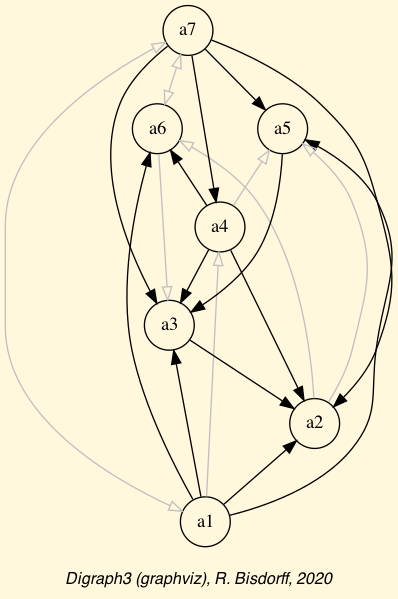
\includegraphics[width=5cm]{Figures/codualOdg.png}
\caption{The codual outranking digraph. It becomes readily clear now from the picture above that both alternatives $a1$  and $a7$ are {\em not outranked\/} by any other alternatives. Hence, $a1$  and $a7$ appear as \emph{weak} \Condorcet winner and may be recommended as potential {\em best decision actions\/} in this illustrative preference modelling exercise.}
\label{fig:3.1}       % Give a unique label
\end{figure}
 
Many more tools for exploiting bipolar-valued outranking digraphs are available in the \Digraph3 resources (see the technical documentation of the {\tt outrankingDigraphs} module and the {\tt perfTabs} module).

 
